% 


\documentclass[twoside]{article}
\setlength{\oddsidemargin}{0.25 in}
\setlength{\evensidemargin}{-0.25 in}
\setlength{\topmargin}{-0.6 in}
\setlength{\textwidth}{6.5 in}
\setlength{\textheight}{8.5 in}
\setlength{\headsep}{0.75 in}
\setlength{\parindent}{0 in}
\setlength{\parskip}{0.1 in}

%
% ADD PACKAGES here:
%

\usepackage{amsmath,amsfonts,graphicx,arydshln}


\newcounter{lecnum}
\renewcommand{\thepage}{\thelecnum-\arabic{page}}
\renewcommand{\thesection}{\thelecnum.\arabic{section}}
\renewcommand{\theequation}{\thelecnum.\arabic{equation}}
\renewcommand{\thefigure}{\thelecnum.\arabic{figure}}
\renewcommand{\thetable}{\thelecnum.\arabic{table}}

%
% The following macro is used to generate the header.
%
\newcommand{\lecture}[4]{
   \pagestyle{myheadings}
   \thispagestyle{plain}
   \newpage
   \setcounter{lecnum}{#1}
   \setcounter{page}{1}
   \noindent
   \begin{center}
   \framebox{
      \vbox{\vspace{2mm}
    \hbox to 6.28in { {\bf EE502 - Linear Systems Theory II
	\hfill Spring 2023} }
       \vspace{4mm}
       \hbox to 6.28in { {\Large \hfill Lecture #1 \hfill} }
       \vspace{2mm}
       \hbox to 6.28in { {\it Lecturer: #2 \hfill } }
      \vspace{2mm}}
   }
   \end{center}
   \markboth{Lecture #1}{Lecture #1}

   \vspace*{4mm}
}

\renewcommand{\cite}[1]{[#1]}
\def\beginrefs{\begin{list}%
        {[\arabic{equation}]}{\usecounter{equation}
         \setlength{\leftmargin}{2.0truecm}\setlength{\labelsep}{0.4truecm}%
         \setlength{\labelwidth}{1.6truecm}}}
\def\endrefs{\end{list}}
\def\bibentry#1{\item[\hbox{[#1]}]}


\newcommand{\fig}[3]{
			\vspace{#2}
			\begin{center}
			Figure \thelecnum.#1:~#3
			\end{center}
	}

% Use these for theorems, lemmas, proofs, etc.
\newtheorem{theorem}{Theorem}[lecnum]
\newtheorem{lemma}[theorem]{Lemma}
\newtheorem{proposition}[theorem]{Proposition}
\newtheorem{claim}[theorem]{Claim}
\newtheorem{corollary}[theorem]{Corollary}
\newtheorem{definition}[theorem]{Definition}
\newenvironment{proof}{{\bf Proof:}}{\hfill\rule{2mm}{2mm}}
\newtheorem{exmp}[theorem]{Ex}

% **** IF YOU WANT TO DEFINE ADDITIONAL MACROS FOR YOURSELF, PUT THEM HERE:

\begin{document}

% Lecture Details
\lecture{16}{Asst. Prof. M. Mert Ankarali}

%%%%%%%%%%%%%%%%%%%%%%%%%%

\section{Minimality of Interconnected Systems}

In this section we shall examine the conditions under which minimality is lost when minimal subsystems are interconnected in various configurations,

\section{Series - Cascade Connection}
		
Consider the following system structure where two sub systems, with transfer functions 
$G_1(s)$ and $G_2(s)$ and associated minimal representations $\left( \begin{array}{c|c} A_1 & B_1 \\ \hline
C_1 & D_1 \end{array} \right)$ and $\left( \begin{array}{c|c} A_2 & B_2 \\ \hline
C_2 & D_2 \end{array} \right)$, connected in series/cascade configuration. 
		
\begin{center}
  \begin{minipage}[h]{0.9\linewidth}
    \begin{center}
      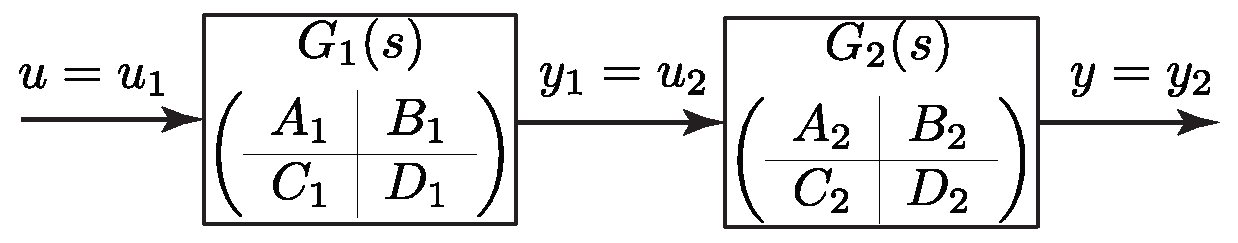
\includegraphics[width=0.9\textwidth]{cascade}
    \end{center}
  \end{minipage}
    \end{center}
		
The transfer function of the connection is simply equal to $G(s) = G_2(s) G_1(s)$. Let $x_1$ and $x_2$
state-variables of the sub-systems, then natural choice of the state variable for the series connection is 
$x = \begin{bmatrix} x_1 \\ x_2 \end{bmatrix}$. Under this definition the state-space representation for the whole system 
can be found as
%
\begin{align*}
A = \left[ \begin{array}{c|c} A_1 & 0 \\ \hline B_2 C_1  & A_2 \end{array} \right]
\, , \, B = \left[ \begin{array}{c} B_1 \\ \hline B_2 D_1  \end{array} \right]
\, , \, C = \left[ \begin{array}{c|c} D_2 C_1 & C_2  \end{array} \right]
\, , \, D = \left[ \begin{array}{c} D_2  D_2  \end{array} \right]
\end{align*}
%
Let's analyze the observability of the connection via PBH test. 


% **** This ENDS THE EXAMPLES. DON'T DELETE THE FOLLOWING LINE:
\end{document}
